\documentclass[12 pt]{article}

% Basic
\usepackage[utf8]{inputenc}
% \usepackage[spanish,mexico]{babel}

% Don't indent paragraphs, leave some space between them
\usepackage{parskip}
\usepackage{enumitem}
\usepackage{graphicx}
\usepackage{subfig}

% Math stuff
\usepackage{amsmath, amsfonts, mathtools, amsthm, amssymb}
\usepackage{breqn}
\usepackage{cancel}
\usepackage{etoolbox}
\usepackage{float}


% For neural networks
\usepackage{tikz}
\usetikzlibrary{matrix,chains,positioning,decorations.pathreplacing,arrows}

% Headers
\usepackage{fancyhdr}
\usepackage{lastpage}
\pagestyle{fancy}
\setlength{\headheight}{40pt}

% Commands
\newcommand\N{\ensuremath{\mathbb{N}}}
\newcommand\R{\ensuremath{\mathbb{R}}}
\newcommand\Z{\ensuremath{\mathbb{Z}}}
\newcommand\Q{\ensuremath{\mathbb{Q}}}
\newcommand\C{\ensuremath{\mathbb{C}}}

%Images
\usepackage{import}
\usepackage{xifthen}
\usepackage{pdfpages}
\usepackage{transparent}

\newcommand{\incfig}[1]{%
    \def\svgwidth{\columnwidth}
    \scalebox{.75}{\import{./figures/}{#1.pdf_tex}}
}

\newtheorem{teo}{Teorema}
\newtheorem{lema}{Lemma}

\newenvironment{solution}
  {\renewcommand\qedsymbol{$\blacksquare$}
  \begin{proof}[Proof]}
  {\end{proof}}
\renewcommand\qedsymbol{$\blacksquare$}


\begin{document}

\lhead{Hyperparameter tuning, Regularization \\ and Optimization}
\rhead{ Deep Learning specialization}
\cfoot{\thepage \ of \pageref{LastPage}}

\section*{Setting up your Machine Learning process}
\subsection*{Train, Dev and Test}

Applied machine learning is a highly iterative process: You start with an idea, you 
experiment with it, get back results and based on the outcome you refine your ideas,
change your choices and repeat the process.

To train a neural network, you have several decisions to make:

\begin{itemize}
    \item Number of laters
    \item Number of hidden units
    \item Learning rate
    \item Activation functions
\end{itemize}

One of the things that determine how quickly you can make progress is how efficiently 
you can go around this cycle. Making good choices in how you set up your training, development, and test sets can make
a huge difference in helping you quickly find a good high performance neural network.

Usually, the rule of thumb in machine learning is a 60\% train, 20\% dev and 20\% test 
partition of the dataset. It's important to consider the size of your dataset, since the
dev and test sets only are to evaluate the performance of a model, it might be 
sufficient to have 10,000 observations in each set, for a dataset of a million observations
that split would be 98\% train, 1\% dev and 1\% test.

Another rule of thumb is to make sure that the dev and test sets come from the same 
distribution.

It might be okay not to have a test set. The goal of a test set is to give an 
unbiased estimate of the error of your algorithm, if you don't need that estimate it's
okay not to have a test set.

\subsection*{Bias and Variance}

\begin{figure}[H]
    \subfloat[High bias]{{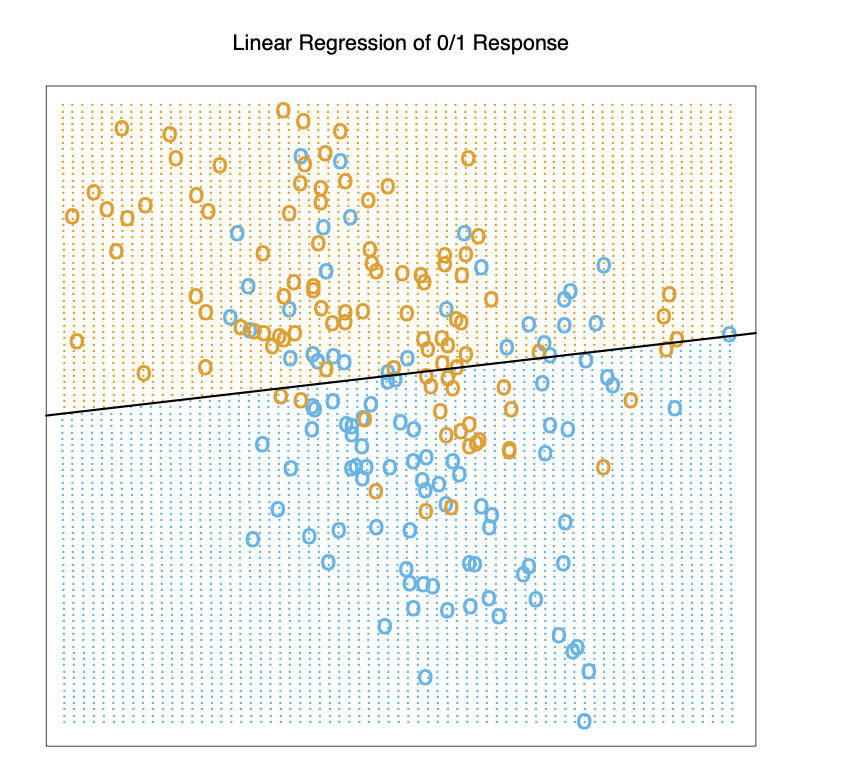
\includegraphics[width=4.5cm]{img/under.png} }}%
    \subfloat[Just right]{{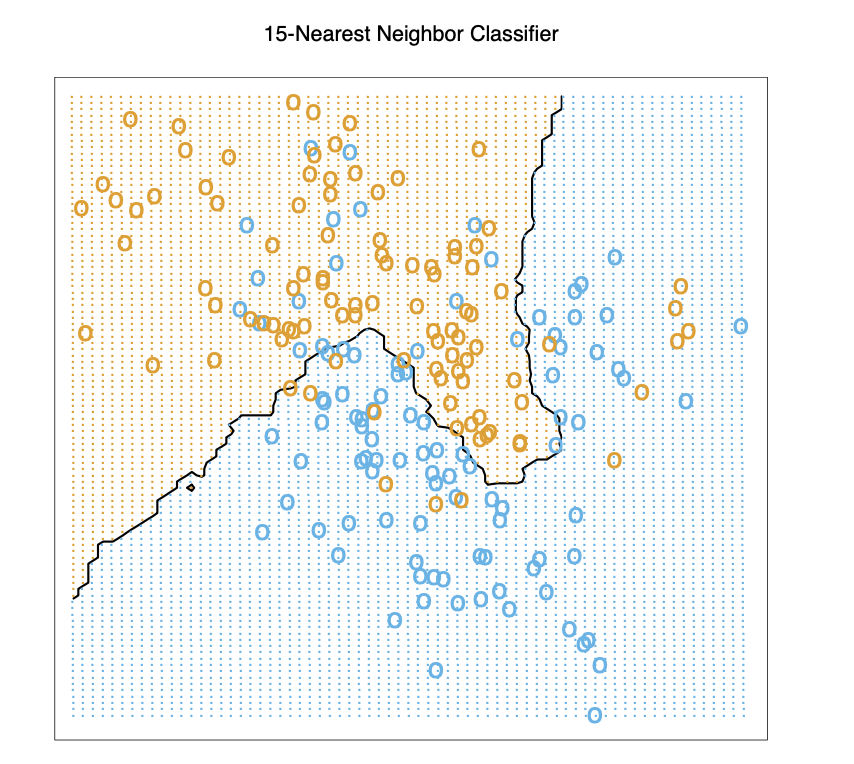
\includegraphics[width=4.5cm]{img/right.png} }}%
    \subfloat[High variance]{{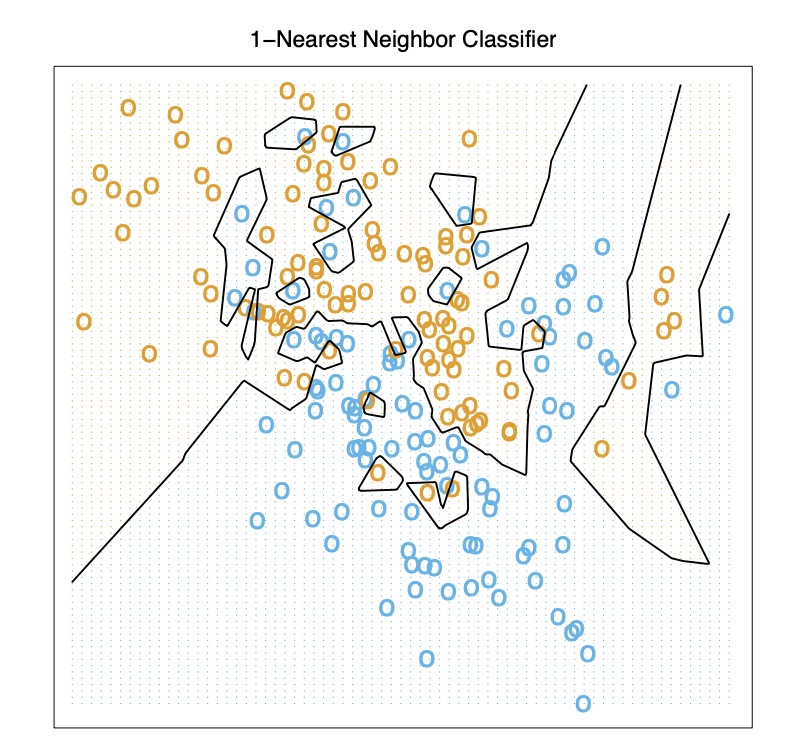
\includegraphics[width=4.5cm]{img/over.png} }}%
    \caption{Bias and variance}
    \label{fig:example}
\end{figure}

Since we have several dimensions it's difficult to plot the decision boundary. We can 
compare the train and dev errors in order to obtain how is our bias and variance:

\begin{itemize}
    \item If the difference between train and dev errors is small we have low variance
    and if it's big we have high variance. 
    \item If the train error is near to the optimal (bayes) error we have low bias 
    and in the other case we have high bias.
\end{itemize}

The following curve ilustrates this tradeoff:

\begin{figure}[H]
    \begin{center}
            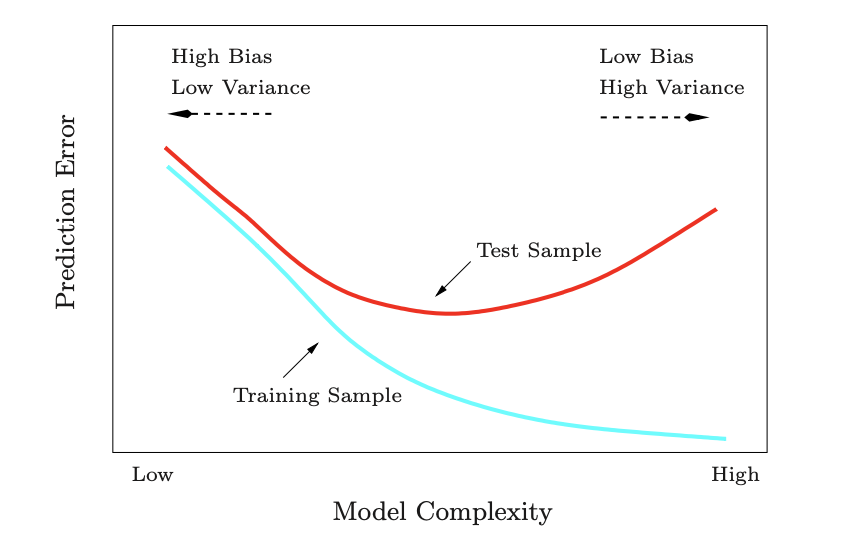
\includegraphics[width=0.6\textwidth]{img/bias-variance.png}
            \caption{Test and training error as a function of model complexity}
        \end{center}
\end{figure}

\subsection*{Basic Recipe for Machine Learning}

If the model has a high bias (train set performance) you can:
\begin{itemize}
    \item Train a bigger network
    \item Train longer
    \item Try a different Neural Network architecture
\end{itemize}

If the model has a high variance (test set performance) you can:
\begin{itemize}
    \item Get more data (if possible)
    \item Regularization
    \item Try a different Neural Network architecture
\end{itemize}

In "traditional" machine learning we speak of the bias-variance tradeoff because we 
could only increase one sacrificing the other. In deep learning is a little bit difference
training a bigger network almost always reduce bias and doesn't increase variance (with
proper regularization) and getting more data almos always reduce variance without 
hurting the bias. This is why deep learning has been so successfull with supervised
learning.

\section*{Regularizing your netural network}
\subsection*{Regularization}

If you have a high variance problem (your neural network is overfitting the data) you 
should try regularization.

Let's begin explaining how regularization works for the logistic regression, we add
the following term to the loss:
\begin{align*}
    J(w,b) = \frac{1}{m} \sum_{i=1}^m L(\hat{y}^{(i)},y^{(i)}) + \color{blue} \frac{\lambda}{2m} \|w\|_p^2
\end{align*}
Where $\lambda$ is called the \textit{regularization parameter} and $\|\dot\|_p$ is the
$p$ norm, the must common regularizations are:
\begin{itemize}
    \item $p=2$ (L2 regularization)
    \item $p=1$ (L1 regularization)
\end{itemize}
L2 regularization is the most common and L1 regularization is used because it makes
the solution sparse.

For a neural network, the regularization looks as follows:
\begin{align*}
    J(w^{[1]},b^{[1]},..., w^{[L]}, b^{[L]}) = \frac{1}{m} \sum_{i=1}^m L(\hat{y}^{(i)},y^{(i)}) + \color{blue} \frac{\lambda}{2m} \sum_{l=1}^L\|W^{[l]}\|^2
\end{align*}
Where $\|W^{[l]}\|$ is the \textit{Frobenius} norm of $W$.

How do you implement gradient descent with this?
\begin{align*}
    dW^{[l]} &= \text{(from backprop)} + \color{blue} \frac{\lambda}{m}W^{[l]} \\
    W^{[l]} &:= W^{[l]} - \alpha dW^{[l]}  \\
    &= W^{[l]}\left(1 - \frac{\alpha \lambda}{m}\right) - \alpha(\text{from backprop})
\end{align*}
That's why this kind of regularization is also known as \textit{weight decay} because
it's just like the original backpropagation but you are multiplying the weght matrix
$W^{[l]}$  by $\left(1 - \frac{\alpha \lambda}{m}\right)$ a number strictly smaller than 
1.

\textbf{Why regularization reduces overfitting?} As lambda gets bigger the penalization 
for $W$ being a large matrix get's bigger and so
the error is bigger. Intuitively as we make $\lambda$ bigger we start making the 
impact of more and more hidden units negligible and therefore obtaining a more
simple network that is therefore less prone to overfitting.

\subsection*{Dropout regularization}
With droput we go through each layer of the network and set some probability $p$ 
of eliminating a node in the neural network so you end up with a much smaller, 
diminished network.
\begin{figure}[H]
    \begin{center}
            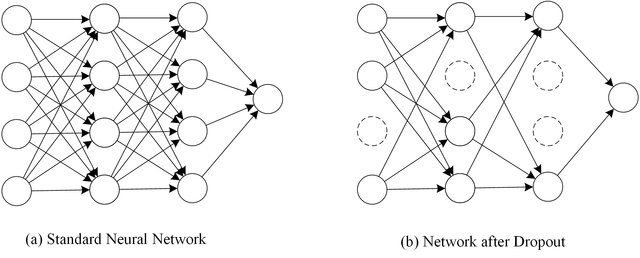
\includegraphics[width=0.9\textwidth]{img/regularization.jpg}
            \caption{Ilustration of regularization}
        \end{center}
\end{figure}

\textbf{Inverted dropout} After removing nodes from the layer $l$ with probability $p$ 
we have to divide $a$ by that probability so that the expected value remains the same.

Notice that each layer can have different probability $p$, for more dense layers you 
might use smaller $p$ (probability to keep a node) and in thinner layers that $p$ can
be bigger or even 1 (no dropout).

Also notice that at test time we shouldn't do any dropout (you would just add noise to your 
predictions)

\textbf{Why does dropout work?} The intuition is that a single unit can't rely solely
in any feature because any one feature could be made zero (because of droput) so 
it has to spread and give a little bit of weight to each incoming feature. By spreading
weights it has an effect of shrinking the squared norm of the weights, similar to L2
regularization.


\subsection*{Other regularization methods}
\textbf{Data augmentation:} Take the examples of an neural network which purpose is image
classification. Then you can flip, zoom, rotate and perform an slight distortion
to each image. The new dataset is bigger and might help reducing to reduce the variance.

\textbf{Early stopping:} By stopping early you have a mid-size $W$ that hasn't still
learned some really specific configurations of the train dataset and therefore overfitting.

Early stopping has one downside, in general you would like to follow the principle of 
orthogonalization, that is, solving different tasks at different times. When training
neural networks we have to worry about optimizing the cost function $J$ and after that
to not overfit. In general we can tackle this two problem in a totally independent way
but early stopping couples this two tasks.

\begin{figure}[H]
    \begin{center}
        \subfloat[Data augmentation]{{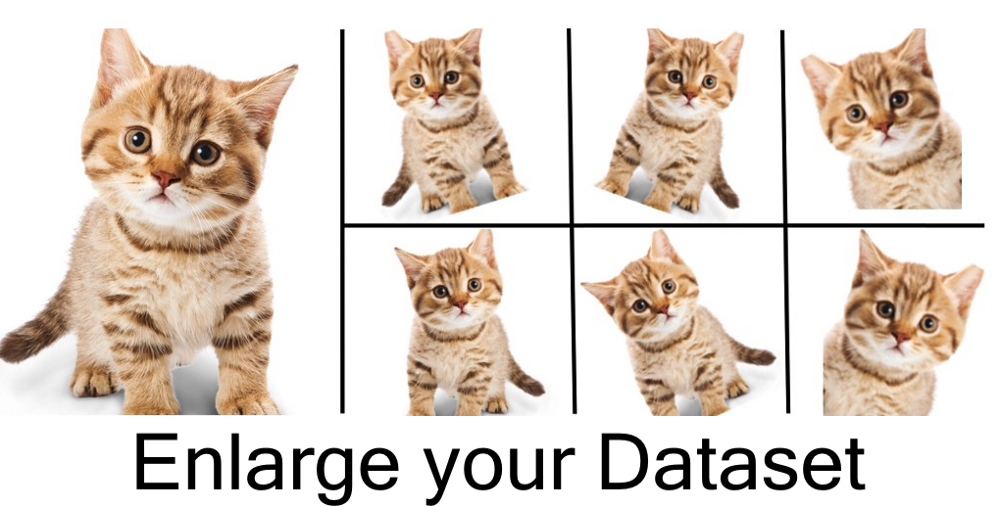
\includegraphics[width=6cm]{img/aumentation.png} }}%
        \quad
        \subfloat[Early stopping]{{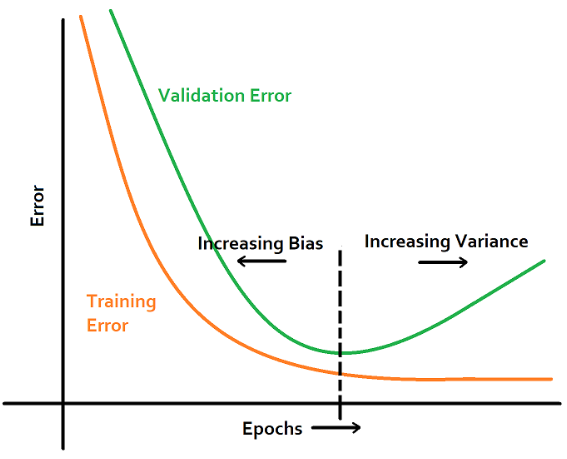
\includegraphics[width=6cm]{img/early-stopping.png} }}%
        \caption{Other regularization methods}
    \end{center}
\end{figure}

A better alternative to early stopping is just using L2 regularization and training for 
as long as possible. The downside of this alternative is that you add another hyperparameter
($\lambda$).

\section*{Setting the optimization problem}
\subsection*{Normalizing inputs}

In general, the cost function of the optimization problem is easier to optimize when 
the training dataset is normalized. To normalize it you have to:
\begin{itemize}
    \item Obtain the dataset mean $\mu = \frac{1}{m}\sum_{i=1}^m x^{(i)}$ and substract 
    it to every observation $x^{(i)} = x^{(i)} - \mu$
    \item Obtain the dataset variance $\mu = \frac{1}{m}\sum_{i=1}^m x^{(i)2}$ and divide
    each observation $x^{(i)} = \frac{x^{(i)}}{\sigma^2}$
\end{itemize}
Notice that you should store this values of $\mu$ and $\sigma^2$ so you can normalize
your test set with this same $\mu$ and $\sigma^2$ values.
\begin{figure}[H]
    \begin{center}
            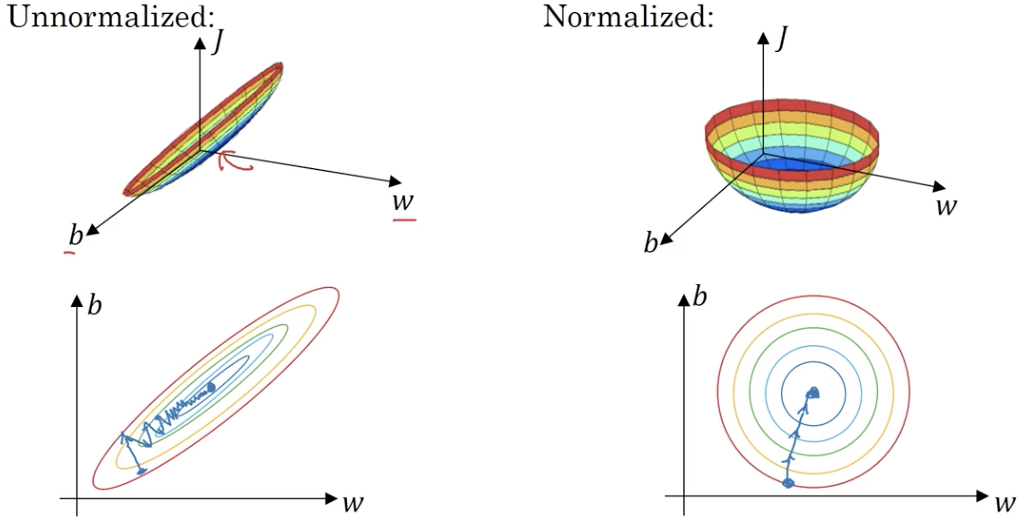
\includegraphics[width=0.9\textwidth]{img/normalized.png}
            \caption{Comparison of countours of the normalized an unnormalized cases}
        \end{center}
\end{figure}

\subsection*{Vanishing / Exploding gradients}




\end{document}
